\chapter{Neural networks}

\section{Artificial neuron}

Artificial neurons, also called perceptrons were developed in the late 1950s and early 1960s, firstly introduced by Rosenblatt in his paper \cite{perceptron}. His idea was to develop a model capable of simulating the activities present in the human brain cell, in order to create artificial intelligence. As it turned out, simulating the brain using such a simple model as the perceptron is impossible. However, later research discovered a considerable potential in the field of classification and regression, which lead to design of modern artificial neural networks as we know them today.

Perceptron\cite{nn_book} is a simple probabilistic model, which takes several weighted real inputs and produces one real output.

\vspace{3mm}

\begin{figure}[h]
\raggedright
\begin{subfigure}{.35\textwidth}
  \centering
  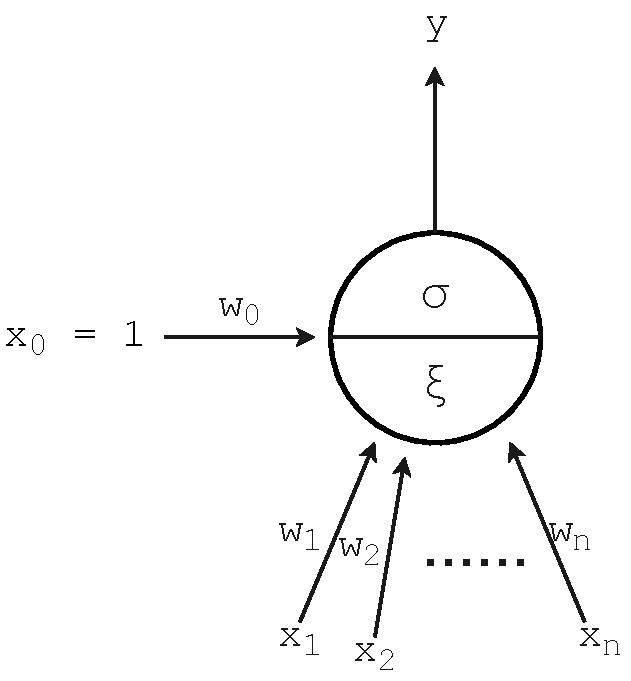
\includegraphics[width=\textwidth]{tex/images/perceptron}
  \caption{Artificial neuron}
\end{subfigure}%
\hfill
\begin{subfigure}{.55\textwidth}
  \centering
  \begin{itemize}

	\item $x_1, \cdots, x_n$ are real \textbf{inputs}
	\item $x_0$ is always equal to 1
	\item $w_0, w_1, \cdots, w_n$ are real \textbf{weights}
	\item $\xi$ is inner \textbf{potential}, \\$\xi = w_0 + \Sigma_{i=1}^n w_i x_i$
	\item $y$ is real \textbf{output} given as \\ $y = \sigma(\xi)$
	\item $\sigma$ is an \textbf{activation function}

	\end{itemize}
\end{subfigure}
\end{figure}

\section{Activation}

An activation function $\sigma: \mathbb{R} \rightarrow \mathbb{R}$ is applied to the inner potential $\xi$, and it defines the output value of perceptron. It introduces a powerful tool into machine learning, and that is \textbf{non-linearity}. Without the activation, the potential by itself is a simple polynomial of a degree of one. That would limit the learning ability of the neural network into being a simple regression model. However, using different activation functions, we can adapt the model to more complicated mappings.

\begin{figure}[h]

\centering
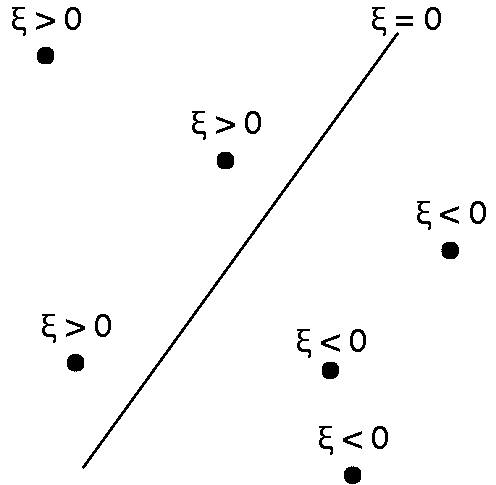
\includegraphics[width=0.45\textwidth]{tex/images/activation-vis}
\caption{Visualization of binary step activation function, which defines a separation hyperplane in n-dimensional space.}
\end{figure}

\noindent
Some desirable properties\cite{wiki:activation} of an activation function include:

\begin{itemize}

\item \textit{non-linearity} - in order to map more complex functions (allows universal function approximations)
\item \textit{continuous differentiability} - necessity for gradient-based optimization methods
\item \textit{range} - for infinite range, training is generally more efficient
\item \textit{monotonicity} - the error surface associated with a single-layer models is guaranteed to be convex
\item \textit{approximates identity near the origin} - initial weights can be randomized with small differences around the origin

\end{itemize}

\noindent
Here are some examples of activation functions\cite{activation_list}:

\subsection*{Identity}

\begin{figure}[H]
\raggedright
\begin{subfigure}{.25\textwidth}
  \centering
  \[ f(x) = x \]
\end{subfigure}%
\begin{subfigure}{.25\textwidth}
  \centering
  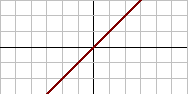
\includegraphics[width=\textwidth]{tex/images/activation/identity}
\end{subfigure}
\end{figure}

\noindent
Effectively remain the potential unchanged. 

\subsection*{Binary step}

\begin{figure}[H]
\raggedright
\begin{subfigure}{.35\textwidth}
  \centering
   \[
f(x) = \begin{cases}
       0 & x < 0 \\
       1 & x \geq 0 \\
     \end{cases} \]
\end{subfigure}%
\begin{subfigure}{.25\textwidth}
  \centering
  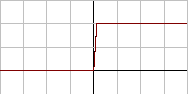
\includegraphics[width=\textwidth]{tex/images/activation/binstep}
\end{subfigure}
\end{figure}

\noindent
Basic activation function, transforms potential into a binary signal. However, this function is not differentiable.
      
\subsection*{Sigmoid}

\begin{figure}[H]
\raggedright
\begin{subfigure}{.28\textwidth}
  \centering
  \[ f(x) = \frac{1}{1 + e^{-x}} \]
\end{subfigure}%
\begin{subfigure}{.25\textwidth}
  \centering
  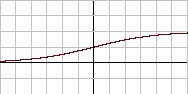
\includegraphics[width=\textwidth]{tex/images/activation/sigmoid}
\end{subfigure}
\end{figure}

\noindent
Smoothened binary step activation function, maps a real value potential into $(0,1)$ range. It introduces non-linearity. One of the most popular functions in the ANN's, mainly in the early era of machine learning. It suffers from vanishing gradient problem\footnote{described in subsection \ref{vanishing_gradient}} and have slow convergence. Furthermore, it is not zero centered, which make optimization harder.
 
\subsection*{TanH}

\begin{figure}[H]
\raggedright
\begin{subfigure}{.5\textwidth}
  \centering
  \[ f(x) = tanh(x) = \frac{(e^x - e^{-x})}{(e^x + e^{(-x)})} \]
\end{subfigure}%
\begin{subfigure}{.25\textwidth}
  \centering
  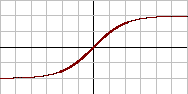
\includegraphics[width=\textwidth]{tex/images/activation/tanh}
\end{subfigure}
\end{figure}

\noindent
Unlike sigmoid, hyperbolic tangent is zero centered. It usually performs better than sigmoid. However, it stills suffers from vanishing gradient problem.

\subsection*{Rectified linear unit (ReLU)}

\begin{figure}[H]
\raggedright
\begin{subfigure}{.35\textwidth}
  \centering
   \[
f(x) = \begin{cases}
       0 & x < 0 \\
       x & x \geq 0 \\
     \end{cases} \]  
\end{subfigure}%
\begin{subfigure}{.25\textwidth}
  \centering
  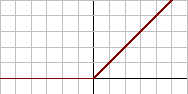
\includegraphics[width=\textwidth]{tex/images/activation/relu}
\end{subfigure}
\end{figure}

\noindent
One of the most popular function in the recent years. As opposed to previous ones, it does not have an issue with vanishing gradient. It is simple and efficient. The limitation is that it should only be used within hidden layers of a model, often combined with softmax in the output layer. It turned out to be very useful in deep learning, where traditional activation functions struggle. For example in \cite{relu_faster}, the convolutional network was able to converge six times faster with ReLU, than with tanh.

\subsection*{Leaky ReLU}

\begin{figure}[H]
\raggedright
\begin{subfigure}{.38\textwidth}
  \centering
  \[
f(x) = \begin{cases}
       0.01x & x < 0 \\
       1 & x \geq 0 \\
     \end{cases} \]  
\end{subfigure}%
\begin{subfigure}{.25\textwidth}
  \centering
  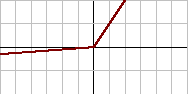
\includegraphics[width=\textwidth]{tex/images/activation/lrelu}
\end{subfigure}
\end{figure}

\noindent
One issue present in ReLU is that it allows the gradient to die off, which is not necessarily a bad thing, though it may result in dead neurons that will never activate on specific data points. To counter this, leaky ReLU's were introduced. To keep the updates alive, they add a small slope into their negative parts (usually with the factor of around 0.01).
   
\subsection*{Randomized ReLU}

\begin{figure}[H]
\raggedright
\begin{subfigure}{.35\textwidth}
  \centering
  \[
f(r, x) = \begin{cases}
       rx & x < 0 \\
       1 & x \geq 0 \\
     \end{cases} \] 
\end{subfigure}%
\begin{subfigure}{.25\textwidth}
  \centering
  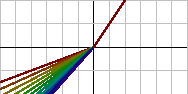
\includegraphics[width=\textwidth]{tex/images/activation/rlrelu}
\end{subfigure}
\end{figure}

\noindent
Another variant of ReLU randomizes the factor in leaky ReLU's.

\subsection*{Softmax}
\label{subsection:softmax}

\begin{figure}[H]
\raggedright
\begin{subfigure}{.25\textwidth}
  \centering
  \[ f(x_j) = \frac{e^{x_j}}{\sum_i e^{x_i}} \]
\end{subfigure}%
\begin{subfigure}{.25\textwidth}
  \centering
  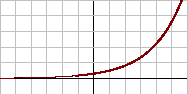
\includegraphics[width=\textwidth]{tex/images/activation/softmax}
\end{subfigure}
\end{figure}

\noindent
Softmax is usually used alongside the ReLU's in the output layer of a deep neural network. It has two nice properties:

\begin{itemize}

\item each value ranges in $[0, 1]$
\item the sum of all values is always 1

\end{itemize}

This is useful when modeling a particular probability distribution. It is used as the estimate of the class distribution for a given input.

\section{Artificial neural network}

Artificial neural network\cite{nn_book} or feed-forward neural network is a directed acyclic graph of artificial neurons organized into several layers, where the following holds:

\begin{itemize}

\item the first layer is called the \textit{input layer}, and the output of neurons is equal to the input vector $\overrightarrow{X}$

\item the last layer is called the \textit{output layer}, and it provides the output $\overrightarrow{Y}$

\item the other layers are called the \textit{hidden layers}

\item outputs of each neuron (except for the output layer) serve as inputs of neurons in the higher layer

\item every two neighboring layers $i$ and $i+1$ make a complete bipartite graph

\item no non-neighboring layers have a connection between them

\end{itemize}

\noindent
In this section we are going to use the following terminology:

\begin{itemize}
  \item every neuron is represented as a distinct natural number (i.e neuron 1, 2, and so forth)
  \item $\xi_i$ is the inner potential of the neuron $i$
  \item $y_i$ is the output of the neuron $i$
  \item $w_{ji}$ is the weight from neuron $i$ to neuron $j$
  \item $j_{\leftarrow}$ is the set of all neurons $i$ such that there exist an edge $w_{ji}$
  \item $j_{\rightarrow}$ is the set of all neurons $i$ such that there exist an edge $w_{ij}$

\end{itemize}

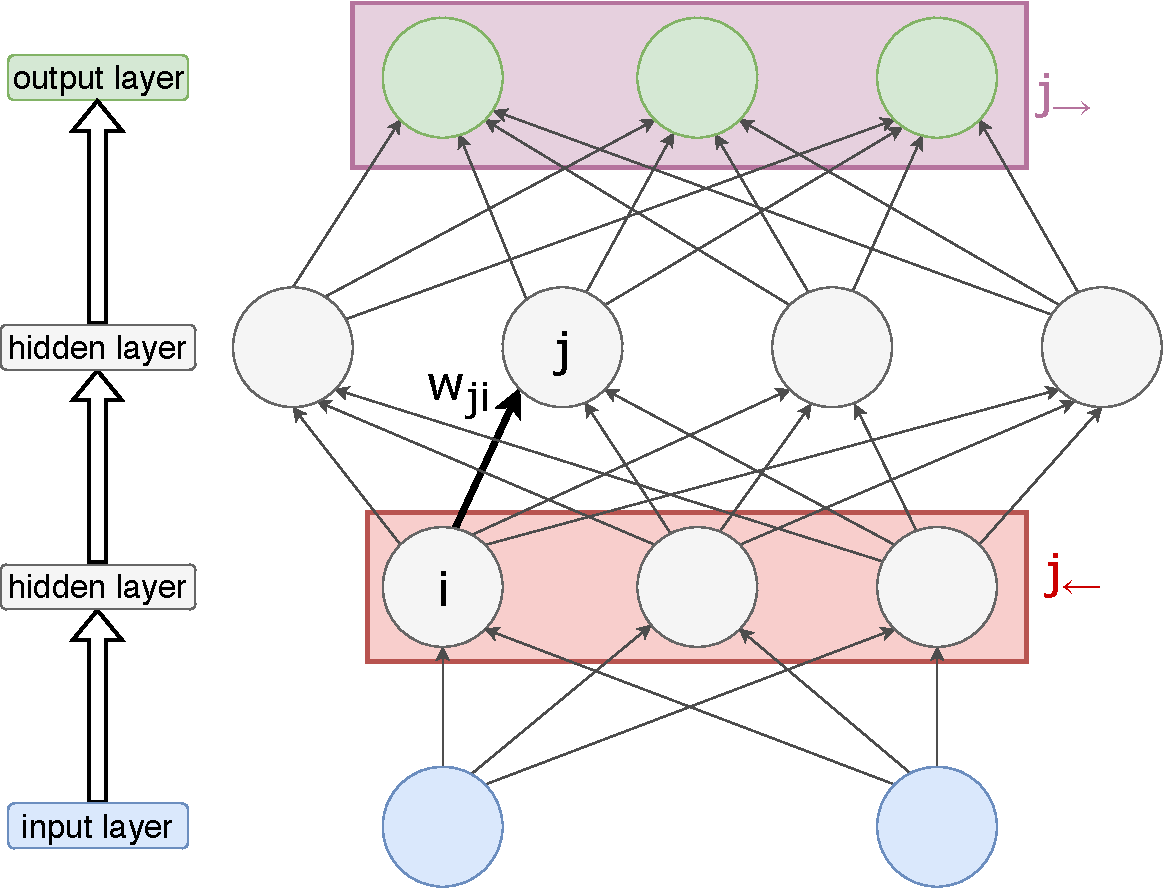
\includegraphics[width=0.8\textwidth]{tex/images/ann}

The neural network is continuously evolving, the states and connections of neurons are changing, weights are adapting. In term of these changes within a period, we can divide the network dynamics into three subcategories:

\begin{itemize}
  \item \textit{organizational} - change in topology
  \item \textit{active} - change in state
  \item \textit{adaptive} - change in configuration
\end{itemize}

\section{Active dynamics}

The values in the input layer are set to the input vector $\overrightarrow{X}$. The forward propagation algorithm is then applied. Starting from the lowest layer, each layer using the output from the previous one updates its neurons. Neuron $j$ updates its inner potential:

$$ \xi_j = w_0 + \sum_{i \in j_{\leftarrow}} w_{ji} y_i $$

The output of neuron $j$ is $y_j = \sigma_j (\xi_j)$. The exception is the input layer, where $y_j = \xi_j$.

\section{Adaptive dynamics}

\textit{Adaptive dynamics} specify the initial configuration of the network and the way, in which the configuration evolves during the training process. Initially are all weights set randomly. In order to update the network weights, we need to define the loss function.

\subsection{Loss function}

At its core, a loss function\cite{loss} is a simple method of evaluating how well the model adapts to the dataset. The higher the loss value is, the more inaccurate the model is. The main goal of the training process is to find the global minima of the loss function. Furthermore, the loss function is differentiable.

Given the set of training data $\tau = \lbrace (\overrightarrow{X_k}, d(\overrightarrow{X_k})) \vert k = 1, \cdots, p \rbrace$, where $\overrightarrow{X_k}$ is a feature, that is fed to the network and $d(\overrightarrow{X_k})$ is a label, that we would like to get as an output from the network.

The loss function is checking the difference between the network's output $\overrightarrow{Y}$ the actual label $d(\overrightarrow{X})$. Hereinafter, we will refer to output layer as OL in this section.

\subsection*{MSE}

One of the simplest loss function used in machine learning methods is \textit{Mean Squared Error} (of MSE for short):

$$ E(\overrightarrow{w}) = \sum_{k=1}^{p} E_k(\overrightarrow{w}) = \sum_{k=1}^{p} \frac{1}{2} \sum_{j \in \text{OL}} (y_j(\overrightarrow{w}, \overrightarrow{X_k}) - d(\overrightarrow{X_k})_j)^2 $$

\noindent
It is widely used in linear regression analysis.

\subsection*{Cross entropy}

Another very popular loss function, which we used is \textit{cross entropy loss}\cite{cross_entropy}. It is a straightforward modification of a basic likelihood function with logarithms over the probability $p$. It penalizes heavily for being very confident and very wrong. 

In order to transform the output vector $\overrightarrow{Y}$ into the probability distribution $P(\overrightarrow{Y})$ we usually use softmax activation function in the output layer (as described in section \ref{subsection:softmax}). With the output transformed into probability vector, we can use the cross entropy:

$$ E(\overrightarrow{w}) =  \sum_{k=1}^{p} E_k(\overrightarrow{w}) = \sum_{k=1}^{p} \sum_{j \in \text{OL}} - d(\overrightarrow{X_k})_j \ln{P(y_j(\overrightarrow{w}, \overrightarrow{X_k}))}$$

\subsection{Gradient descent and backpropagation}

Stochastic gradient descent\cite{deep_learning_SGD} and its variants are probably the most used optimization algorithms for machine learning in general. To update weights according to the given loss function, we need to compute the gradient at any given point on the function in the hyperplane. The gradient vector points towards the closest local minimum. It is the direction in which we want to update our weights.

The learning algorithm is computing the sequence of weight vectors $\overrightarrow{w}^{(0)}, \overrightarrow{w}^{(1)}, \overrightarrow{w}^{(2)}, \cdots$, where:

\begin{itemize}

\item $\overrightarrow{w}^{(0)}$ is the initial vector set randomly (usually weights close to 0)
\item in the $(i+1)$-th step is $\overrightarrow{w}^{(t+1)}$ computed as:

\begin{flalign}
\notag w_{ji} & = w_{ji}^{(t)} + \Delta w_{ji}^{(t)} & \\
\notag \Delta w_{ji}^{(t)} & = - \epsilon(t) \frac{\partial E}{\partial w_{ji}}(\overrightarrow{w}^{(t)}) & 
\end{flalign}

\item $\Delta w_{ji}^{(t)}$ is the weight difference in the step $(t+1)$ and $0 < \epsilon(t) < 1$ is the learning rate in the step $(t+1)$

\begin{flalign}
\notag \frac{\partial E}{\partial w_{ji}} & = \sum_{k=1}^p  \frac{\partial E_k}{\partial w_{ji}} & \\
\notag \frac{\partial E_k}{\partial w_{ji}} & = \frac{\partial E_k}{\partial y_j} \cdot \sigma_{j}^{'}(\xi_j) \cdot y_i & 
\end{flalign}

\begin{flalign}
\notag \frac{\partial E_k}{\partial y_j} &  = 
     \begin{cases}
       y_j - d(\overrightarrow{X_k})_j & \quad\text{for } j \in \text{ OL} \\
       \sum_{r \in j^{\rightarrow}} \frac{\partial E_k}{\partial y_r} \cdot \sigma_{r}^{'}(\xi_r) \cdot w_{rj} & \quad\text{otherwise} \\
     \end{cases} &
\end{flalign}

\end{itemize}

\noindent
While the feed-forward phase was evaluated from the input layer towards the output layer, the weight update is done in the different direction. Starting from the output layer, we are using the partial derivatives from the layer above to evaluate the current layer. This process is also known as \textit{backpropagation}.

There are two general types of weight update algorithms:

\subsection*{Batch algorithm}

It is the approach described above. It takes a batch of data points in each and computes only one weight update for all of these points together. The advantages include:

\begin{itemize}

\item the direction of the descent is identical to the gradient descent vector
\item parallelism is easy to implement - data point losses can be computed secludedly

\end{itemize}

\noindent
Some of the problems are:

\begin{itemize}

\item memory consumption
\item redundant data do not add any information to the gradient
\item is more likely to end up in some local minimum than online algorithm

\end{itemize}

\subsection*{Online (stochastic) algorithm}

Online algorithm is essentially a batch algorithm, where batch consists of only one data point\footnote{point can be taken deterministically or at random (thus stochastic)}. Instead of the whole batch, we update the weight for each data point:

$$ \Delta w_{ji}^{(t)} = - \epsilon(t) \frac{\partial E_k}{\partial w_{ji}}(\overrightarrow{w}^{(t)}) $$

\noindent
Therefore it is not taking the path of gradient descent exactly, but rather "zigzag" alongside the gradient descent vector. The advantages include:

\begin{itemize}

\item it has a better chance of escaping the local minimum than batch algorithm
\item less memory consumption
\item faster (especially on redundant data)

\end{itemize}

\noindent
The problems of online algorithm:

\begin{itemize}

\item not suitable for parallelism
\item can behave weirdly, because it is not taking the direct path to minimum

\end{itemize}

\section{Issues}

There are widely known issues when working with neural networks, which have to be taken into consideration when working with models. In this section, we will mention just a couple, which we encountered and had to deal with.

\subsection{Data set split}

Very simple, but very crucial mechanism used in machine learning is to define three separate sets (\textit{train}, \textit{valid} and \textit{test}). These sets have to be disjoint. It is necessary to use \textit{valid} set during the training process and different \textit{test} set for model evaluation, once the model is trained. The reason behind is that always the model will have a slight bias towards the \textit{valid} test compared to the independent \textit{test} set.

\subsection{Vanishing gradient problem}

\label{vanishing_gradient}

The \textit{vanishing gradient problem}\cite{vanishing_gradient} is a difficulty found in training ANN's. The problem is, that in some cases the gradient will be vanishingly small with the impact on weight update. It gets more apparent with many-layered feedforward networks as well as with recurrent networks. Activation functions such as \textit{hyperbolic tangent} and \textit{sigmoid} suffer from vanishing gradient, while others like ReLU or Leaky ReLU do not.

\section{Model evaluation}
\label{nn-metrics}

After the training process, a huge emphasis is put into the model evaluation. With the incorrect evaluation methods, even the poorly trained model can have a good overall score. Several factors have to be taken into consideration like the uneven distribution of data classes, false negatives, and false positives or the classification interchanging between two groups.

\subsection{Confusion matrix}

In the field of machine learning and specifically the problem of statistical classification, a \textit{confusion matrix}\cite{conf_matrix} is a two-dimensional matrix $n \times n$, where $n$ is the number of classes. Each row of the matrix represents the instances in a predicted class while each column represents the instances in an actual class. It is the most verbose output of the evaluation. We can see the wrongly classified classes, but also the classes which the model misclassified into. 

\begin{figure}[h]
\centering
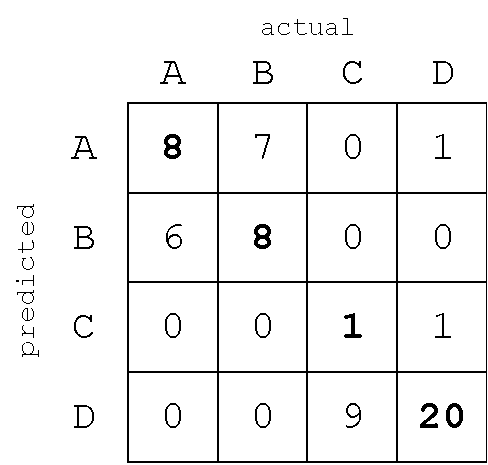
\includegraphics[width=0.37\textwidth]{tex/images/conf_matrix}
\caption{Example of a classification matrix.}
\label{conf_matrix}
\end{figure}

\noindent
In Figure \ref{conf_matrix}, we can see the classification matrix for four classes. The correctly classified cases lie on the main diagonal. Several observations about our model can be seen. First of all, our model almost always misclassifies class \textit{C} as class \textit{D}. Furthermore, the model has difficulties distinguishing between classes \textit{A} and \textit{B} (it would be a good idea to merge these classes).

\subsection{Metrics}

There are four standard metrics for model evaluation: \textbf{accuracy}, \textbf{precision}, \textbf{recall} and \textbf{f1}. Let us take simple binary confusion matrix:

\vspace{3mm}

\begin{table}[h]
\centering
\begin{tabular}{|r|c c|}

\hline 
& $A$ & $\neg A$ \\
\hline 
$A$ & TP & FP \\
$\neg A$ & FN & TN\footnote{true positive / false positive / false negative / true negative} \\
\hline

\end{tabular}

\end{table}

\begin{align*}
\textit{accuracy } & = \frac{TP + TN}{TP + FP + FN + TN} & \\
\textit{precision } & = \frac{TP}{TP + FP} & \\
\textit{recall } & = \frac{TP}{TP + FN} & \\
\textit{F1 } & = \frac{2 \times \textit{ precision } \times \textit{ recall}}{\textit{precision } + \textit{ recall}} &
\end{align*}



